% Compile with pdflatex to regenerate renalsafe-architecture.pdf.
\documentclass[tikz,border=2pt]{standalone}
\usetikzlibrary{arrows.meta}
\definecolor{ink}{HTML}{183643}
\definecolor{teal}{HTML}{19645E}
\definecolor{pale}{HTML}{EEF5F4}
\definecolor{grayblue}{HTML}{576974}
\begin{document}
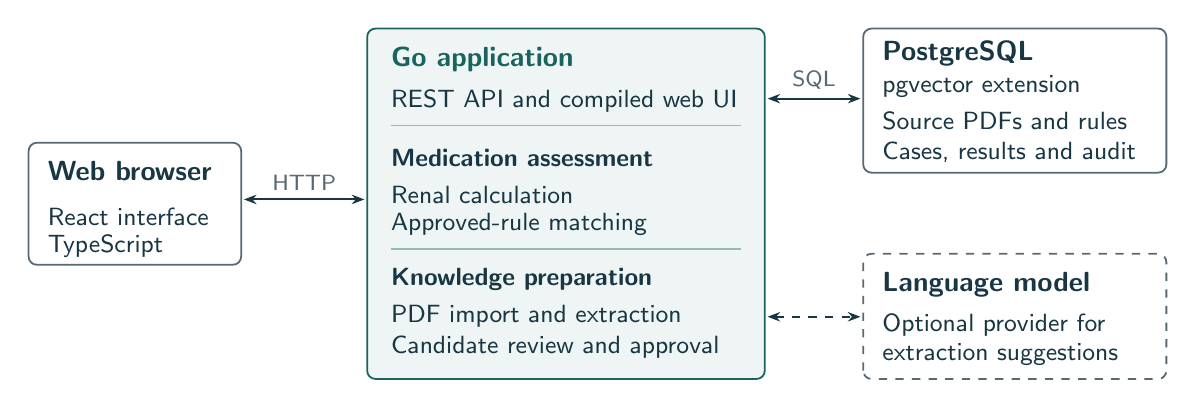
\begin{tikzpicture}[
    x=1cm, y=1cm, font=\sffamily\small, text=ink,
    box/.style={draw=grayblue, rounded corners=3pt, line width=.65pt},
    wire/.style={{Stealth[length=1.6mm]}-{Stealth[length=1.6mm]}, draw=ink,
                 line width=.7pt, shorten <=1pt, shorten >=1pt},
    title/.style={font=\sffamily\bfseries\normalsize, anchor=west},
    detail/.style={anchor=west, font=\sffamily\small},
    linklabel/.style={font=\sffamily\footnotesize, text=grayblue, inner sep=1pt}
]
  % Left: the browser is outside the deployment containers.
  \draw[box] (0,1.45) rectangle (2.70,3.00);
  \node[title] at (.12,2.64) {Web browser};
  \node[detail] at (.12,2.06) {React interface};
  \node[detail] at (.12,1.68) {TypeScript};

  % Centre: both workflows run in one Go process.
  \filldraw[box, fill=pale, draw=teal] (4.30,0) rectangle (9.35,4.45);
  \node[title, text=teal] at (4.48,4.05) {Go application};
  \node[detail] at (4.48,3.53) {REST API and compiled web UI};
  \draw[teal!45] (4.60,3.22) -- (9.05,3.22);
  \node[detail, font=\sffamily\bfseries\small] at (4.48,2.81) {Medication assessment};
  \node[detail] at (4.48,2.34) {Renal calculation};
  \node[detail] at (4.48,1.97) {Approved-rule matching};
  \draw[teal!45] (4.60,1.65) -- (9.05,1.65);
  \node[detail, font=\sffamily\bfseries\small] at (4.48,1.27) {Knowledge preparation};
  \node[detail] at (4.48,.79) {PDF import and extraction};
  \node[detail] at (4.48,.40) {Candidate review and approval};

  % Right: shared persistent storage and the optional provider.
  \draw[box] (10.60,2.62) rectangle (14.45,4.45);
  \node[title] at (10.72,4.13) {PostgreSQL};
  \node[detail] at (10.72,3.72) {pgvector extension};
  \node[detail] at (10.72,3.28) {Source PDFs and rules};
  \node[detail] at (10.72,2.88) {Cases, results and audit};
  \draw[box, dashed] (10.60,0) rectangle (14.45,1.59);
  \node[title] at (10.72,1.20) {Language model};
  \node[detail] at (10.72,.68) {Optional provider for};
  \node[detail] at (10.72,.31) {extraction suggestions};

  \draw[wire] (2.70,2.28) -- node[linklabel, above=2pt] {HTTP} (4.30,2.28);
  \draw[wire] (9.35,3.56) -- node[linklabel, above=2pt] {SQL} (10.60,3.56);
  \draw[wire, dashed] (9.35,.79) -- (10.60,.79);
\end{tikzpicture}
\end{document}
